\documentclass[english]{article}

%% ---------------------------- packages ------------------------------------ %%
\usepackage[T1]{fontenc}
\usepackage{natbib} % citations
\usepackage{csvsimple, longtable, makecell, booktabs}
\usepackage{pgfplotstable}
\usepackage{rotating} % to rotate tables
\usepackage{verbatim}
%% tikz packages
\usepackage{tikz}
\usetikzlibrary{trees, arrows, shapes.geometric, positioning}
\usepackage{tikzpeople}
\usepackage{forest}
\usepackage{standalone}
%% text packages
\usepackage{siunitx} % fake ° symbol \ang{}
\usepackage[super]{nth} % for 1st, 2nd etc. \nth{}
\usepackage{hyperref}
\usepackage{listings} % code highlighting
\usepackage{color}

%% ---------------------------- commands ------------------------------------ %%
\newcommand{\standartox}{STANDARTOX}
\newcommand{\epa}{EPA ECOTOX data base}
\newcommand{\rpackage}{http://139.14.20.252:3838/etox-base-shiny/}
\newcommand{\git}{https://github.com/andreasLD/etox-base}
\newcommand{\gitapp}{https://github.com/andreasLD/etox-base-shiny}
\newcommand{\ecfifty}{EC\textsubscript{50}}

%% ---------------------------- code ---------------------------------------- %%
\definecolor{dkgreen}{rgb}{0,0.6,0}
\definecolor{gray}{rgb}{0.5,0.5,0.5}
\definecolor{mauve}{rgb}{0.58,0,0.82}

\lstset{frame=tb,
  language=R,
  aboveskip=3mm,
  belowskip=3mm,
  showstringspaces=false,
  columns=flexible,
  basicstyle={\small\ttfamily},
  numbers=none,
  numberstyle=\tiny\color{gray},
  keywordstyle=\color{blue},
  commentstyle=\color{dkgreen},
  stringstyle=\color{mauve},
  breaklines=true,
  breakatwhitespace=true,
  tabsize=3
}


\listfiles


\begin{document}


\title{Standartox: Standardising toxicity data}

\author{Andreas Scharm{\"u}ller\textsuperscript{1{*}},
        Verena C. Schreiner\textsuperscript{1},
        Ralf B. Sch{\"a}fer\textsuperscript{1}}

\maketitle
%\thispagestyle{fancy}

1. Institute of Environmental Sciences, University of Koblenz-Landau Fortstraße 7, 76829 Landau, Germany {*}corresponding author(s):
Andreas Scharm{\"u}ller (andschar@protonmail.com)

\begin{abstract}
%%5This is a manuscript template for Data Descriptor submissions to \emph{Scientific
%%Data} (http://www.nature.com/scientificdata). The abstract must be
%%no longer than 170 words, and should succinctly describe the study,
%%the assay(s) performed, the resulting data, and the reuse potential,
%%but should not make any claims regarding new scientific findings.
%%No references are allowed in this section. 

<WRITE ABSTRACT>

\end{abstract}
\pagebreak

%%%%%%%%%%%%%%%%%%%%%% 01 Introduction
\section{Summary}
An increasing number of chemicals such as pharmaceuticals, pesticides and synthetic hormones are in daily use all over the world. In Europe alone, some 100,000 chemicals are estimated to be in current use, whereof 30,000 are produced in quantities larger than one ton per year \citep{breithaupt_costs_2006}. Except for pesticides that are released into the environment deliberately, most chemicals enter the environment as a result of their use through different paths (e.g. atmospheric emission and deposition or discharge through wastewater) \citep{schwarzenbach_challenge_2006}. In the environment, chemicals can adversely affect populations and communities and in turn related ecosystem functions \citep{rhind_anthropogenic_2009, clements_community_2009, hallmann_declines_2014, barracaracciolo_pharmaceuticals_2015, johnston_review_2015, hallmann_more_2017, sanchez-bayo_worldwide_2019}. Ultimately, this may compromise natures contribution to human well-being, for example the ecosystem services clean drinking and irrigation water, food and climate regulation \citep{peters_review_2013, vandersluijs_neonicotinoids_2013, barracaracciolo_pharmaceuticals_2015, yamamuro_neonicotinoids_2019}. Pollution with man-made chemicals has been identified as one of three major environmental problems for which research gaps hamper the derivation of planetary boundaries, i.e. thresholds beyond which irreversible state shifts may occur \citep{steffen_anthropocene_2007, steffen_planetary_2015}. \citet{bernhardt_synthetic_2017} argue that the knowledge gap how chemicals affect populations, communities and in turn ecosystem functions and services, may impede the accomplishment of the Sustainable Development Goals of the United Nations. Even highly regulated chemical compounds such as pesticides have been shown to cause strong adverse effects on organisms, such as birds \citep{hallmann_declines_2014} or fish \citep{yamamuro_neonicotinoids_2019}, questioning the current regulation efforts \citep{schafer_future_2019}. To evaluate the risks from chemicals for ecosystems data on their toxicity, which is typically produced in standardised ecotoxicological laboratory tests is required. For example, \citet{morrissey_neonicotinoid_2015} used ecotoxicological test results from 49 insect and crustacean species to evaluate the effect of neonicotinoids, an insecticide class on the aquatic ecosystem. Also, \citet{malaj_organic_2014} compiled experimental toxicity test results for 223 various chemical compounds to assess the health of freshwater ecosystems in Europe. Similarly, permissible environmental concentrations are often derived from these test data, typically by a combination with safety factors to account for uncertainties, thereby mostly relying on a few, well tested standard organisms, such as the water flea \textit{Daphnia magna}, the fathead minnow \textit{Pimephales promelas}, the microalga \textit{Raphidocelis subcapitata} to name a few, although researchers have conducted experiments on a much greater variety of organisms. Given that data sets with large numbers of analysed chemicals are becoming increasingly available, ecotoxicity data are pivotal for regulatory risk assessment (RA) and science. To date, only few initiatives exist that aim to create a public resource of harmonized and quality controlled ecotoxicological data, such as the United States Environmental Protection Agency ECOTOXicology knowledgebase (ECOTOX) (~1,000,000 test results, ~13,000 taxa, ~12,000 chemicals) \citep{elonen_ecotoxicology_2018}, the German Environmental Agency's Information System Ecotoxicology and Environmental Quality Targets (ETOX) \citep{umweltbundesamt_etox_2019} or the Pesticide Property Data Base (PPDB) (~ 2000 chemicals) \citep{lewis_international_2016}. The former two compile all available test results into a database. However, for many chemicals, multiple ecotoxicity values are available for the same test organism, which can vary strongly. Hence, these databases can contain multiple entries for the same test without quality information and with different units, hampering reproducible science if different values are selected for studies. 


The PPDB database is confined to pesticides and provides harmonised and quality controlled data for a few selected test organisms, thereby ignoring vast amounts of data for other species and chemicals. Moreover, data analyses often require links to additional data resources, for example to append additional chemical and species information (e.g. chemical properties, habitat of species), which calls for more automated procedures. We therefore developed Standartox, a tool and database that aims to overcome the limitations of other databases by continuously incorporating the ever-growing number of test results in an automated process workflow that ultimately leads to single aggregated data points for a specific chemical-organism test combination. Standartox makes use of the publicly available and quarterly released EPA ECOTOX database \citep{usepa_ecotox_2019} and restricts the data to three commonly used endpoints in ecotoxicology (i.e. XX50, LOEX \& NOEX) and further harmonises and cleans the data, leading to roughly 600,000 ecotoxicological test results including 8000 chemicals, tested on about 7873 taxa. The tool allows user to filter test results according to several parameters, e.g. refining a search for ecotoxicity data on organisms occurring in specific habitats or regions of the world. Above all, Standartox aggregates ecotoxicological test results in a standardized way, by calculating the minimum, the geometric mean and the maximum of the result for each chemical for user-defined test parameters. This relaxes the commonly occurring problem of the variability of multiple ecotoxicological test results and which to choose for chemical risk assessment (CRA). Hence, Standartox provides the basis for reproducible science and combines information from different sources to simplify the derivation of more advanced risk indicators such as Species Sensitivity Distributions (SSD) and Toxic Units (TU), which represent two prominent concepts to assess effects on organisms in ecotoxicology \citep{posthuma_species_2002, kefford_definition_2011, schafer_effects_2011}. Besides aggregating ecotoxicological test results, Standartox provides a concise overview of the status of tested chemicals, allowing the identification of potential research gaps. Standartox comes with two front-ends, a web application (APP): \url{standartox.uni-landau.de} and a R \citep{rcoreteam_language_2017} package \textit{standartox}, which accesses a application programming interface (API) providing convenience structures and thereby largely reducing processing time for users.

Both access pathways allow for the same filters and aggregation methods (Table \ref{tab:app-parameters}) to be applied and access the same data set. 

%%%%%%%%%%%%%%%%%%%%%%%%%%%%%%%%%%%%%%%%%% IDEAS %%%%%%%%%%%%%%%%%%%%%%%%%%%%%%%%%%%%%%%%%
\iffalse

\item \citep{fernandes_lethal_2016} example for ecotoxicological tests


\item Put in citation \citep{hartung_chemical_2009} ? which claims that REACH won't meet their assumptions and say 54 million vertebrate animals are needed for tests that would cost €9.5 billion over the next ten years. I.e 20 times more animals, 6 times the costs in comparison to the official estimates 


For dicussion:
Showed general decline in biodiversity and biomass, but no or not much causes: \citep{butchart_global_2010, hallmann_more_2017, seibold_arthropod_2019} 

Direct effect of chemicals:
include \citep{yamamuro_neonicotinoids_2019} % ecosystem services, food webs

- gerneral stuff about small water bodies: \citep{riley_small_2018}


\item standardized toxicity values
    
\item reproducible research % TODO mention much more often!
    
\item time saving
\fi    

%%%%%%%%%%%%%%%%%%%%%%%%%%%%%%%%%%%%%%%%%% OLD %%%%%%%%%%%%%%%%%%%%%%%%%%%%%%%%%%%%%%%%%%%
\iffalse

A large number of chemicals such as pharmaceuticals, pesticides and synthetic hormones are in daily use all over the world with insufficient knowledge about possible adverse effects on the environment. In Europe alone some 100,000 chemicals are estimated to be in current use, whereof 30,000 are produced in quantities larger than one ton per year \citep{breithaupt_costs_2006}. Chemicals are brought to the environment deliberately - as it is the case of pesticides, or arrive therein as a byproduct from other processes (e.g. atmospheric emissions or wastewater) \citep{schwarzenbach_challenge_2006}. Ecosystems provide essential services to human societies such as drinking and irrigation water, food and climate regulation. These services are products of different ecosystem functions that crucially depend on the integrity of the populations and communities that drive these ecosystem functions. However, besides habitat degradation, climate change and nutrient enrichment, pollution with man-made chemical toxicants threatens these populations and communities in various ways which are currently not fully understood \citep{steffen_anthropocene_2007}. Pollution with man-made chemical toxicants was indeed identified as one of three major environmental problems for which research gaps hamper the derivation of planetary boundaries, i.e. thresholds beyond which irreversible state shifts may occur \citep{steffen_anthropocene_2007}. Bernhardt et al. \citet{bernhardt_synthetic_2017} argue further that the knowledge gap how chemicals effect populations and communities and hence ecosystem functions and ecosystem services, would also impede society's ability to accomplish the Sustainable Development Goals of the United Nations. According to Breithaupt \citet{breithaupt_costs_2006} less than one percent of chemicals released to the environment are thoroughly tested. Although for some chemicals advanced and standardized \citep{oecd_oecd_2018} test methods have been developed, ecotoxicological tests for a lot of chemicals, especially newly emerging ones remain scarce and if existent, the information is represented sparsely and in inconsistent formats. \citep{gessner_fostering_2016}. Therefore we developed a data base that collects, processes and aggregates ecotoxicological tests results in order to subsequently publish it in an harmonized form as a web application - the \etoxbase{} tool: \href{http://139.14.20.252:3838/etox-base-shiny/}. This should facilitate researchers the access to ecotoxicological test results and support modern chemical risk assessment (CRA) workflows. The \etoxbase{} makes use of ecotoxicological test data, obtained from the ECOTOXicology knowledgebase (ECOTOX) created by the U.S. Environmental Protection Agency (EPA). ECOTOX collects raw, non harmonized ecotoxicological test data on aquatic and terrestrial wildlife as well as plants and publishes it on a quarterly basis. By the time of writing it contained 926,108 test results, comprising 11,685 chemicals tested on 12,668 different species \citep{elonen_ecotoxicology_2018}. The collected ecotoxicological test data contain a variety of measured endpoints such as Effective Concentrations (\ecfifty{}) values, No-observed effect concentrations (NOEC) or lowest observed effect concentrations (LOEC). Likewise the data set contains different effect measures such as mortality, intoxication and growth as well as a multiplicity of test durations ranging from seconds to weeks or even years. The \etoxbase{} aggregates this information according to the user's inputs. These can then be used for the derivation of risk indicators such as Species Sensitivity Distributions (SSDs) \citep{posthuma_species_2002} and Toxic Units (TUs), which represent two prominent concepts to assess effects on organisms in ecotoxicology. The former combines toxicity data of several organism groups towards a chemicals to estimate effects on biotic communities, the latter refers to effects of a specific organism (group) towards a chemical. The two concepts are widely used in ecotoxicology \citep{kefford_definition_2011, schafer_effects_2011} since the allow for a comparison of toxicities across multiple chemicals and biological communities, respectively. Although performed on one and the same organism and chemical, outcomes of different ecotoxicological tests vary greatly due to differences in test parameters, genetic differences in individual populations or other irrepressible factors making a selection of appropriate test results for CRA laborious. The \etoxbase{} aims to relief this process and provide single toxicity values for organism, chemical and test duration combinations. The \etoxbase{} downloads every new version of the ECOTOX data base and performs several quality checks, e.g. unit harmonization, and cleaning steps on it. Hence, new scientific test results are constantly incorporated. Additionally the \etoxbase{} queries chemical- and organism-specific variables from other open data bases to fill information gaps such as water solubility, organism habitat or regional occurrence patterns in the ECOTOX data base.

\fi



%%%%%%%%%%%%%%%%%%%%%% 02 Data Description
\section{Data Description}
Standartox constitutes a collection of 600,000 quality checked ecotoxicological test results comprising roughly 8000 distinct chemicals and 8000 taxa that allows for the retrieval of single toxicity equivalents. It is build on the ECOTOX database \citep{usepa_ecotox_2019} and the data are processed to clean and harmonise entries to retrieve comparable toxicity endpoints. Subsequently, filter and aggregation methods are provided to allow for the retrieval of single toxicity equivalents for specific experimental conditions. The underlying ECOTOX database is updated quarterly and provides on average 5228 (2014 - 2019) new toxicity entries with each update. As soon as a new update of ECOTOX is available, Standartox is directly built in an automated way and therefore incorporates new data steadily. Standartox comes with a version control to guarantee reproducibility, meaning that once derived Standartox estimates can be retraced at a later stage, although new data might have updated the estimates already. Users can reach Standartox via a web application and an R-package (standartox) that accesses an application programming interface (API) providing the possibility of scriptable requests.

\subsection{Filters}
The data can be restricted to the three endpoint groups, namely half maximal effective/lethal concentration/dose values (e.g. EC50, LD50), henceforth abbreviated as XX50, lowest observed effect levels/concentrations (LOEC/L), henceforth abbreviated as LOEX and no observed effect levels/concentrations (NOEL/C), henceforth abbreviated as NOEX (Table \ref{tab:endpoints-conflate}). Standartox allows the ecotoxicity data to be filtered by effect groups (e.g. mortality, population, growth) (Fig. \ref{fig:stx-parameters}B) and concentration types (e.g. formulation, active ingredient) as well as test durations (in hours). In addition to these test-specific parameters, Standartox data entries can be filtered by chemical-specific parameters such as the CAS number and chemical roles (e.g. pesticides, metals, drugs) (Fig. \ref{fig:stx-parameters}B) and classes (e.g. organochlorine, triazine) (Fig. \ref{fig:stx-parameters}C). Furthermore, the Standartox data can be refined to organism-specific parameters, such as the organism habitat (e.g. freshwater, marine, terrestrial) (Fig. \ref{fig:stx-parameters}E), their occurrence regions (e.g. Europe, South America) (Fig. \ref{fig:stx-parameters}F) as well as different taxonomic levels.

\begin{figure}[h!]
    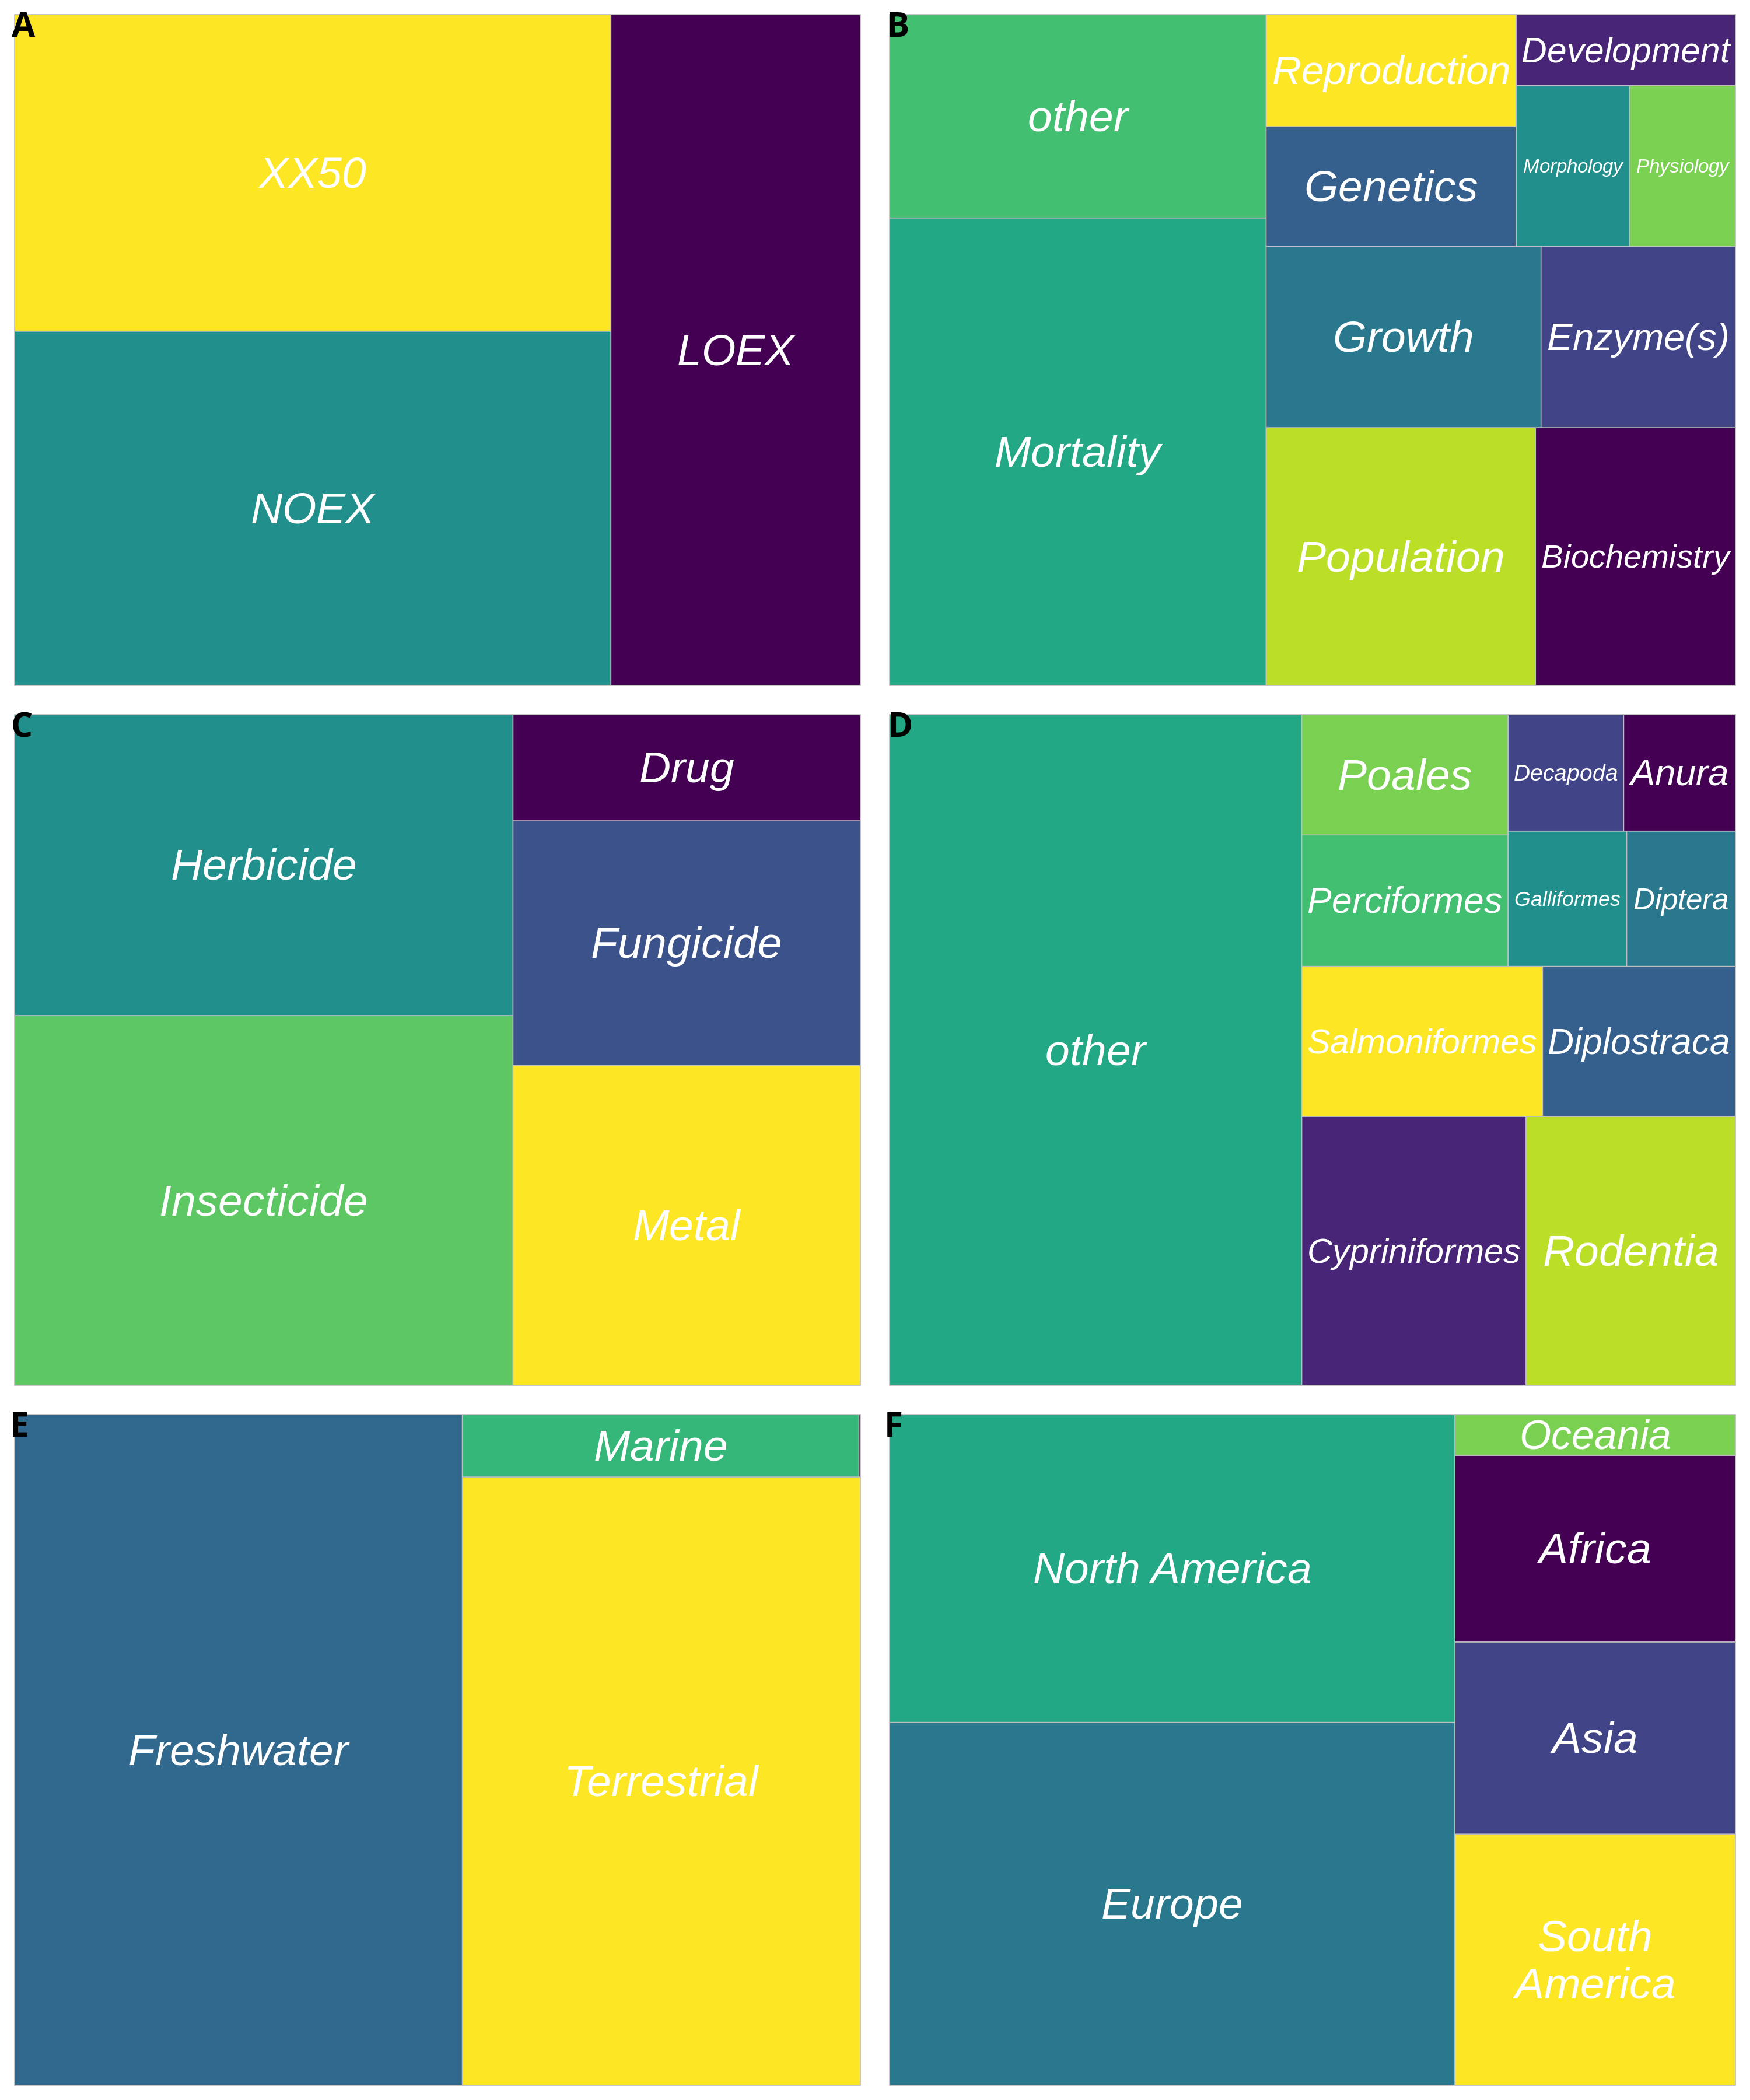
\includegraphics[width=1.0\textwidth]{article/figures/standartox_parameters.png}
    \caption{Share of 10 most frequent entries for the parameters effect group (A), chemical role (B), chemical class (C), taxonomic order (D), organism habitat (E) and organism occurrence region (F) in Standartox.}
    \label{fig:stx-parameters}
\end{figure}

\subsection{Aggregation}
Typically, species exhibit a differential sensitivity towards chemicals (Fig. \ref{fig:stx-variability}A). Moreover, multiple ecotoxicity values are available for individual species-chemical combinations and these can also exhibit high variability due to several factors such as durations of ecotoxicity tests (Fig. \ref{fig:stx-variability}B), experimental conditions and physiology and genetic strain of the test individuals or populations. To aggregate multiple ecotoxicity values into a single value on the desired taxonomic level (e.g. for an individual species, across species of a genus or family), and chemical grouping (e.g. across all pesticides), Standartox provides several aggregation methods including the minimum, the maximum and the geometric mean allowing to aggregate the filtered data set. The geometric mean is preferred in comparison to the arithmetic mean, because it is considerably less influenced by outliers and is suitable for skewed data. Also, the geometric mean is preferable over the median, because the median completely ignores the influence of large or small values, making it unreliable for small data sets. In the course of the aggregation process, outliers that exceed 1.5 times the interquartile range are flagged to caution Standartox users. However, since the geometric mean is relatively robust against outliers, they are not removed automatically from the aggregation. Overall, aggregation with Standartox allows to reduce the between-study variability when toxicity data are aggregated.

\begin{figure}[h!]
    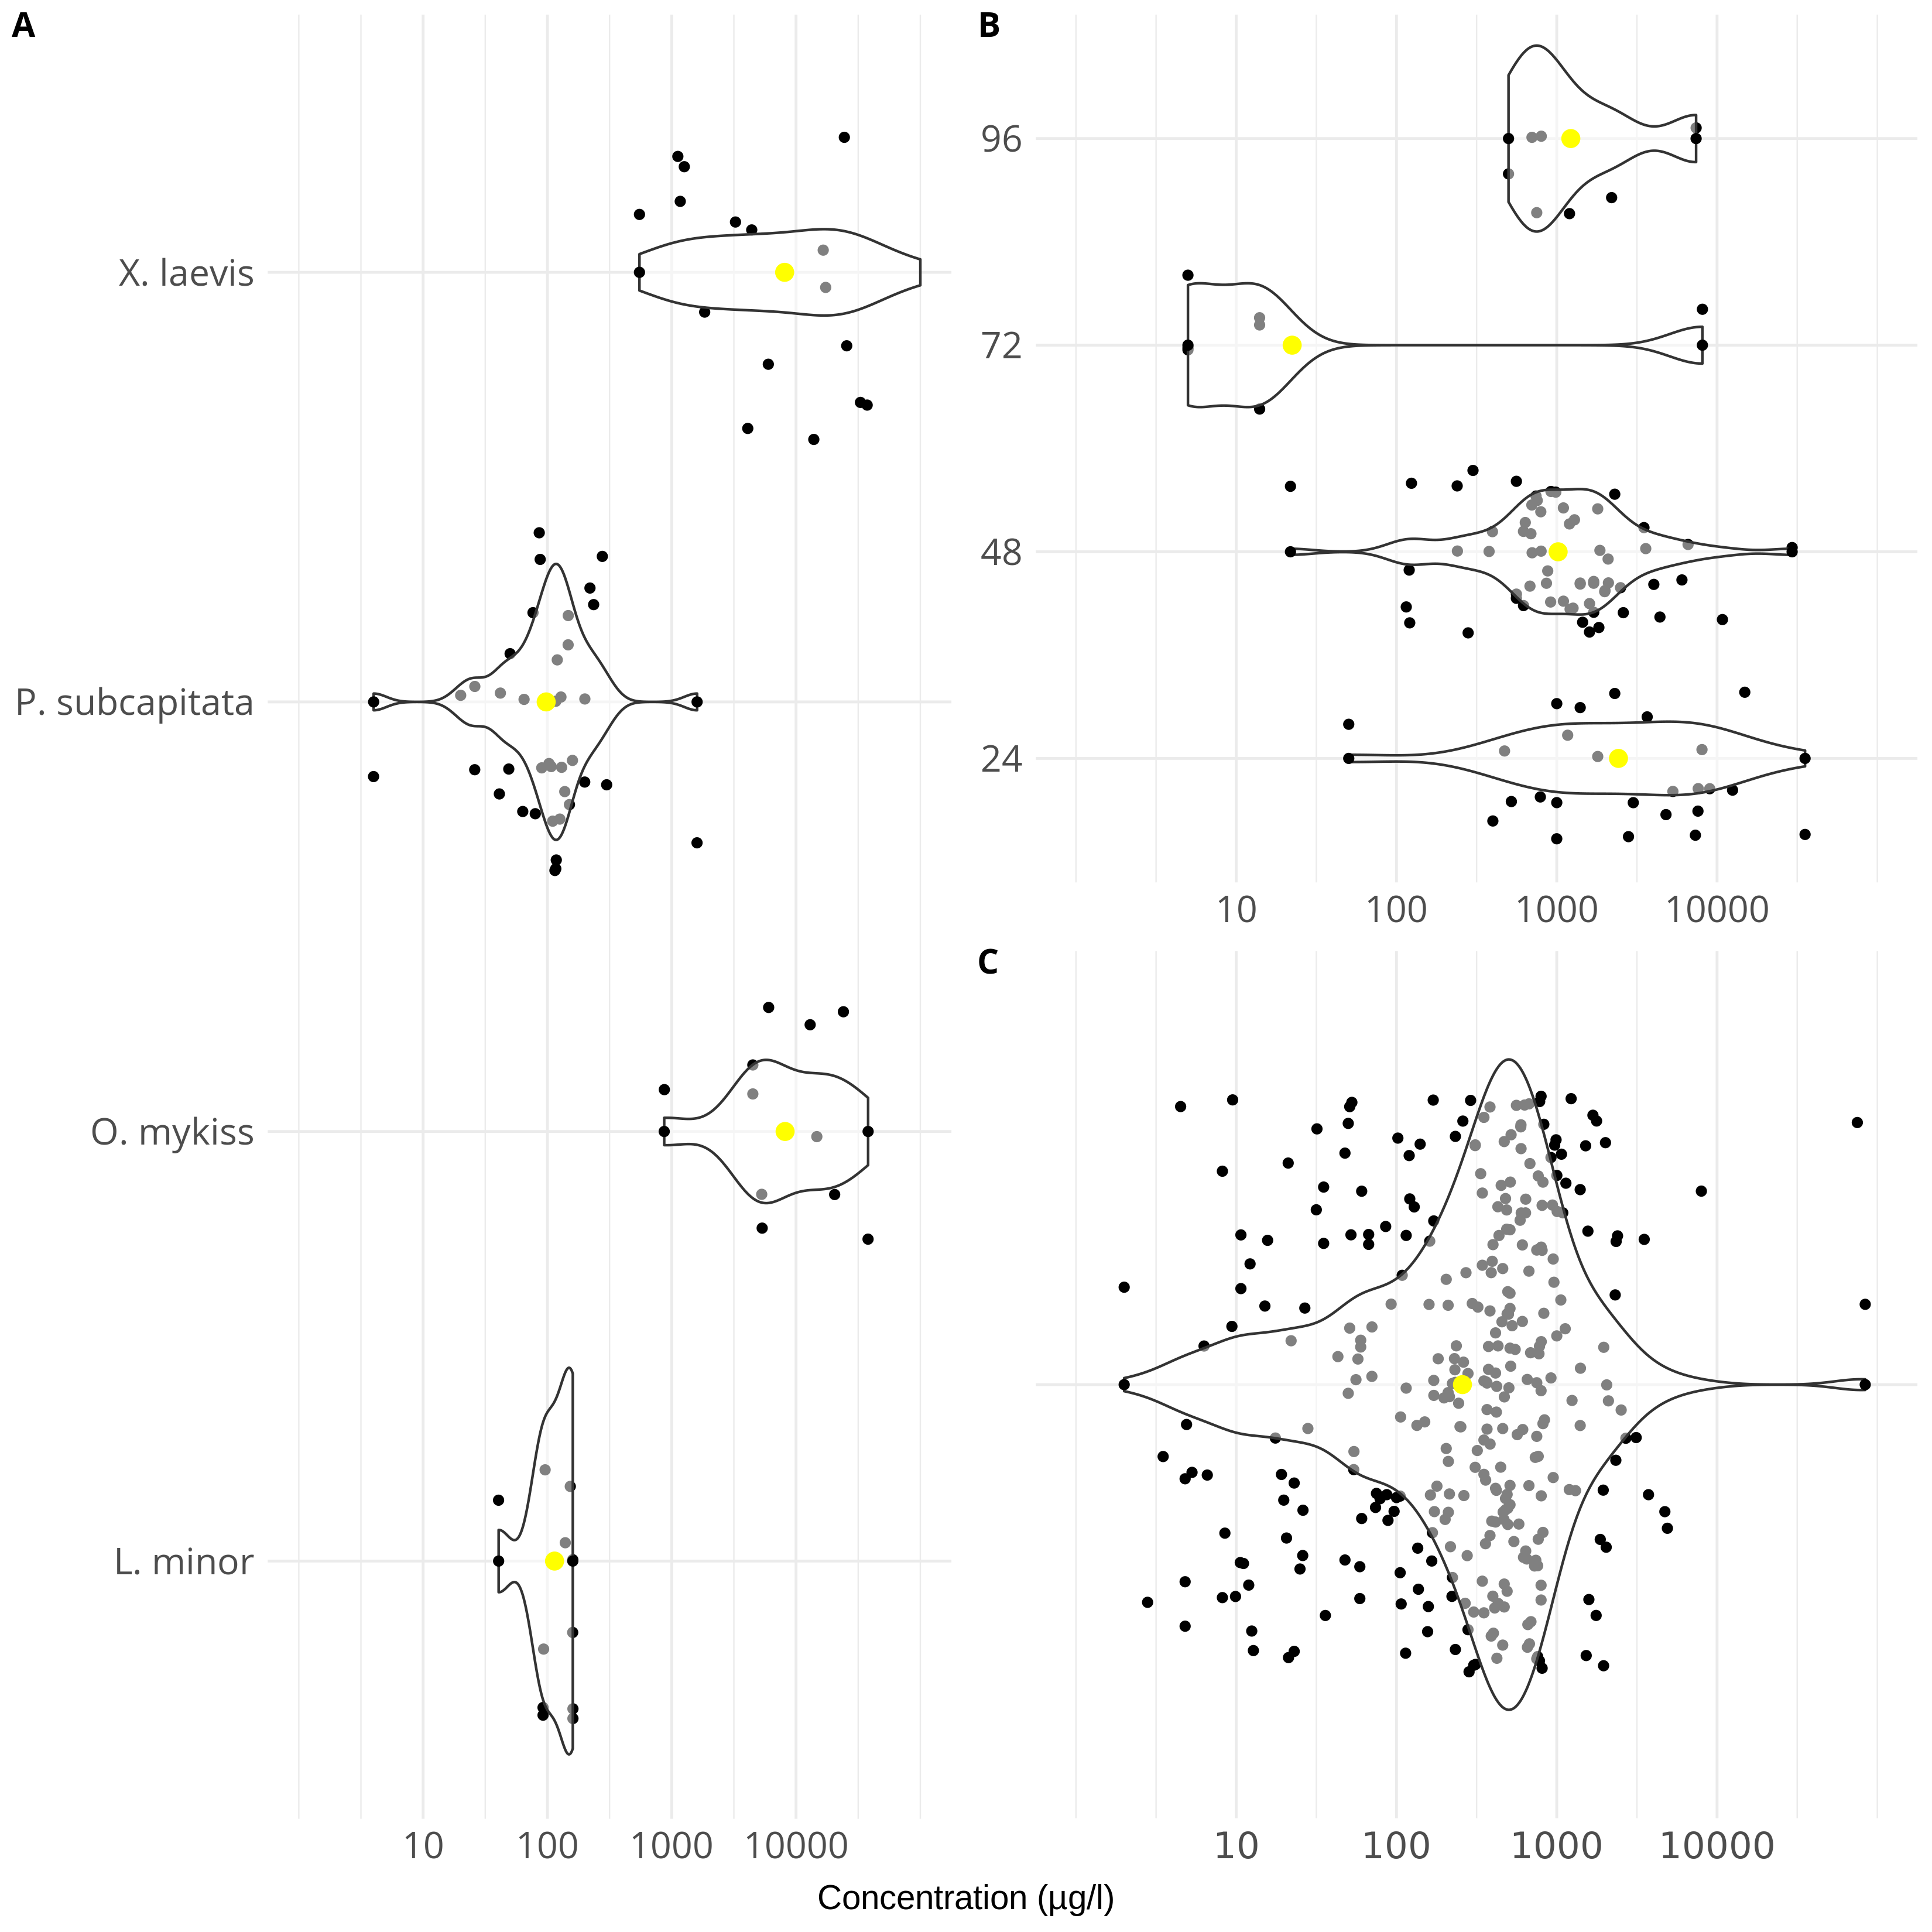
\includegraphics[width=1.0\textwidth]{article/figures/results_variability.png}
    \caption{Violin plots of the variability of test results (EC\textsubscript{50}) in Standartox because of different species (i.e. \textit{Xenopus laevis} - Amphibia, \textit{Raphidocelis subcapitata} - Algae, \textit{Oncorhynchus mykiss} - fish, \textit{Lemna minor} - invertebrate) to the chemical atrazine tested for 96 h (A), different durations of toxicity tests with zinc sulfate and \textit{Daphnia magna} (B) and unaccountable variability of cupric sulfate tested on \textit{Pimephales promelas} for 96 h (C). Purple dots depict Standartox geometric mean estimates and black dots show un-aggregated values for each group. To facilitate readability, data points are randomly scattered along a hypothetical y-axis and are greyed out within the violins.}
    \label{fig:stx-variability}
\end{figure}

\subsection{Accuracy Assessment}
To validate Standartox results we compared the aggregated results using the geometric mean to values from other databases. The PPDB provides ecotoxicity data on a few selected species from chemical risk assessment that have been manually quality controlled through expert judgement \citep{lewis_international_2016}. The vast majority of aggregated values (91 \%) of Standartox lie within one order of magnitude of the corresponding PPDB values (n = 3601). This would increase to 92.7 \%, when restricting the comparison to Standartox values where data from at least five experiments were available. Similarly, we compared Standartox to ecotoxicity values for \textit{D. magna} from the ChemProp \citep{ufzdepartmentofecologicalchemistry_chemprop_2019} software, which estimates LC\textsubscript{50} values via quantitative structure-activity relationship (QSAR) models \citep{schuurmann_quantitative_2011} We found that  95 \% of Standartox values lie within one order of magnitude of the Chemprop (n = 179) vlaues. However, the difference is not necessarily an indication of lower quality of Standartox estimates but may also reflect the wider range of experimental conditions for which data are available in the database underlying Standartox as well as inaccurate predictions for QSAR models, respectively (Figure \ref{fig:standartox_ppdb_diff}).

\begin{figure}[h!]
    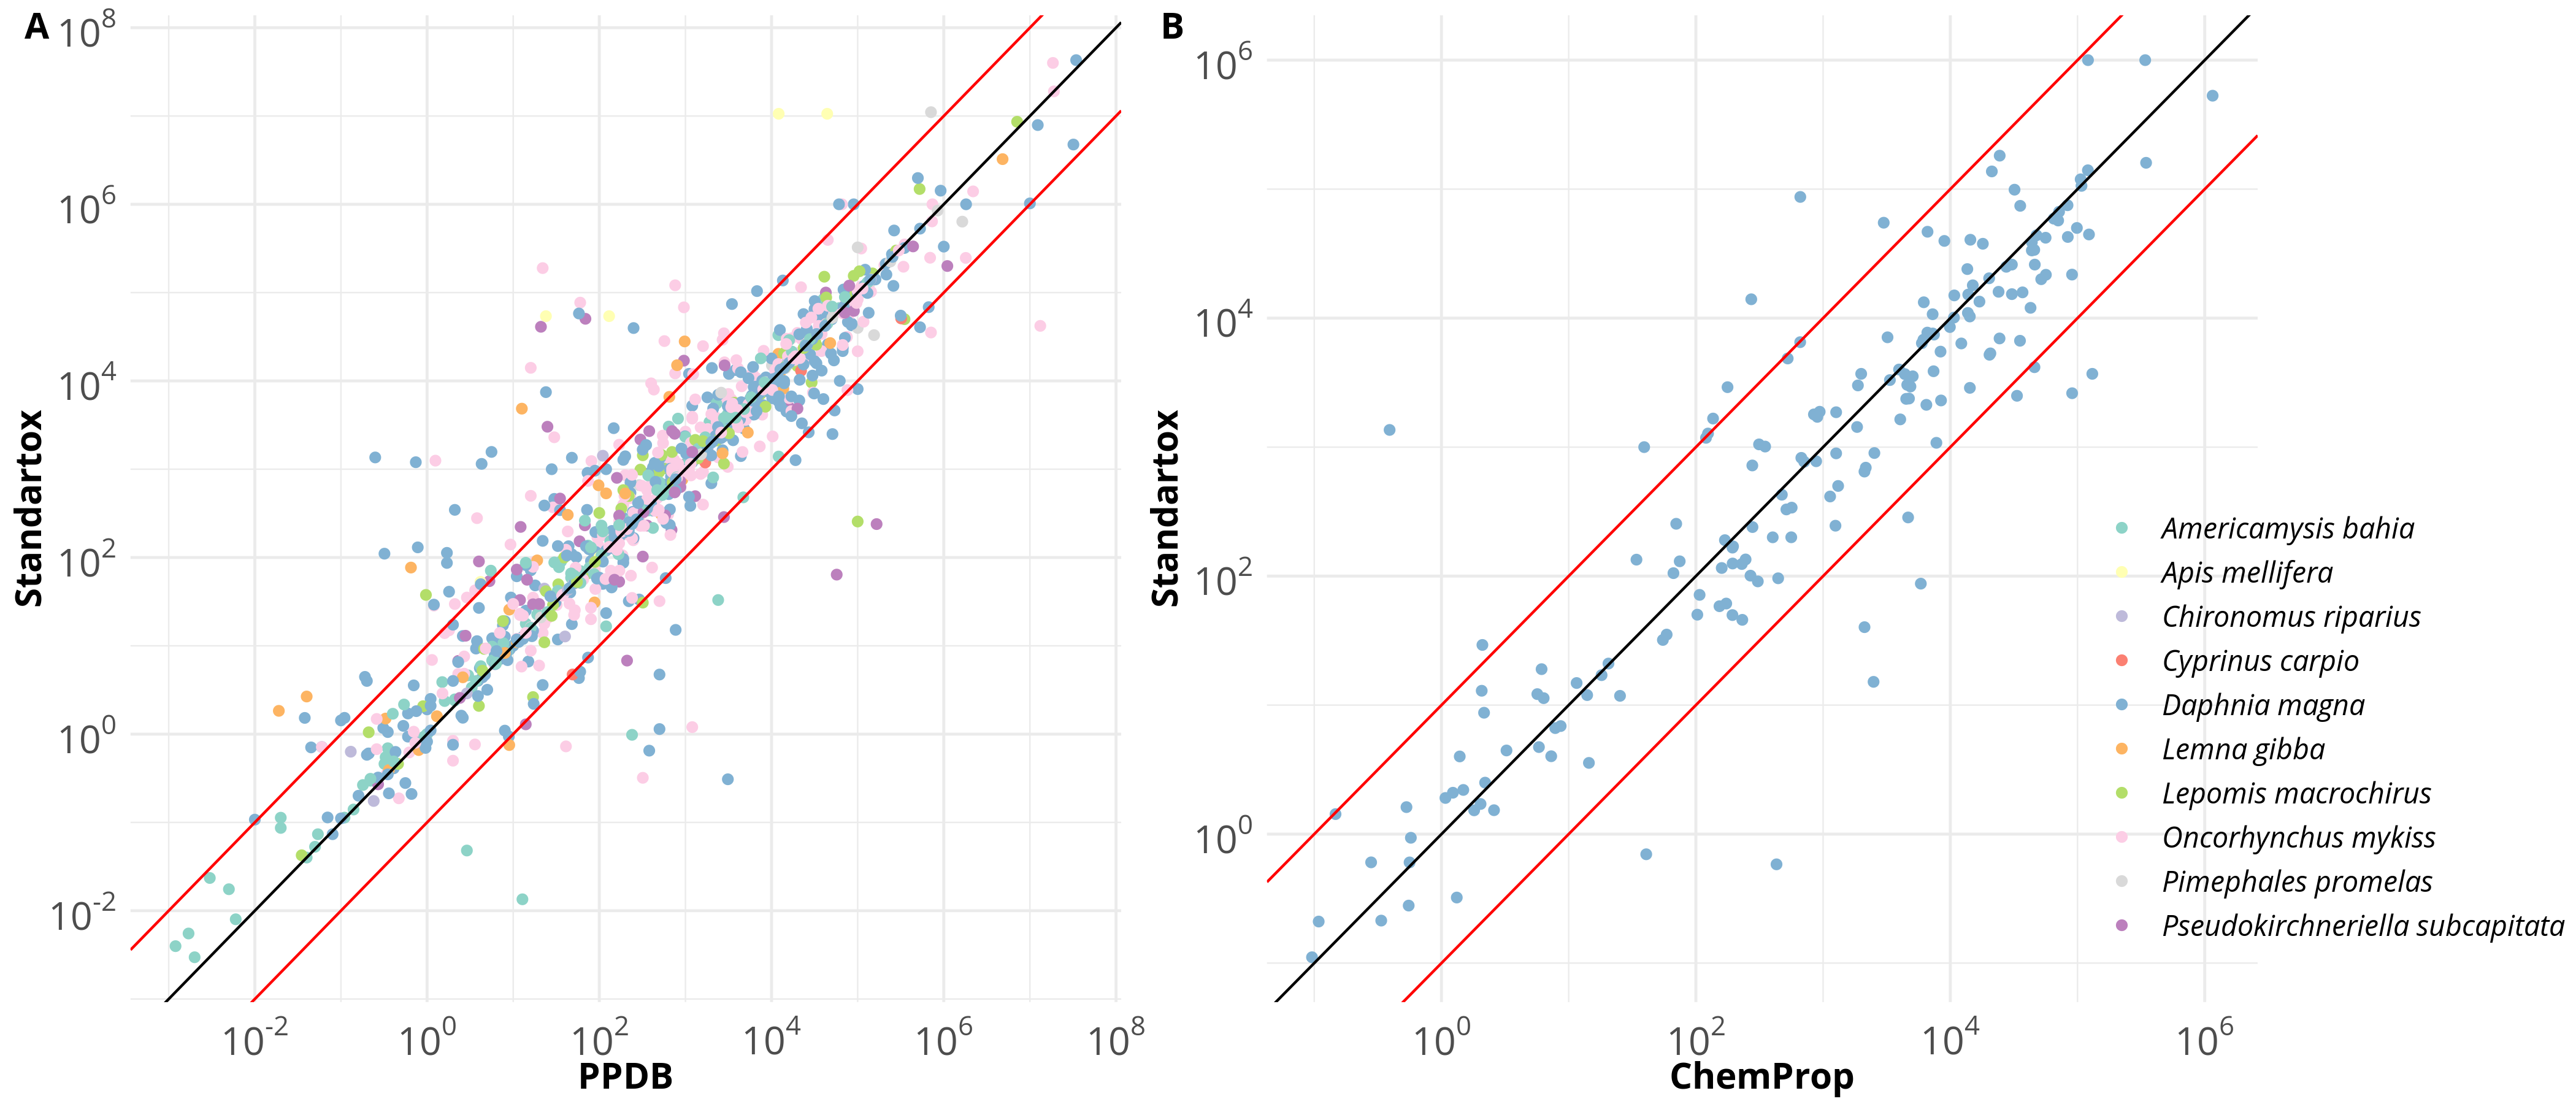
\includegraphics[width=1\linewidth]{article/figures/gg_ppdb_stan_compare_continous.png}
    \caption{Comparison between Standartox and (A) PPDB and (B) ChemProp values. The black lines indicate identity and red lines mark a divergence of a factor of 10. Compared species are color coded.}
    \label{fig:standartox_ppdb_diff}
\end{figure}

\subsection{Perspectives}
Novel predictive frameworks incorporating chemical mode of action and species traits emphasize the need for holistic and automated analyses of large-scale ecotoxicological data \citep{malaj_evolutionary_2016, vandenberg_modeling_2019}. Indeed, the increasing amount of data from ecotoxicological tests and experiments that is becoming available has elicited several initiatives to harmonize these data. These initiatives partly aim for overlapping goals, yet have limitations or objectives that discriminate them from Standartox:

Comptox, is a web tool published by the EPA which, similar to Standartox allows for filtering test results, the retrieval of additional chemical information and the estimation of toxicity equivalents, such as 48 h \textit{Daphnia magna} LC\textsubscript{50} values. However, toxicity estimations are limited to standard organisms (e.g. \textit{Daphnia magna}), and the tool lacks the possibility for automated retrieval \citep{williams_comptox_2017}.

The EnviroTox database which also uses, amongst others the ECOTOX database as an input has recently been published \citep{healthandenvironmentalsciencesinstitutehesi_envirotox_2019, connors_creation_2019}. In contrast to Standartox, EnviroTox  is restricted to selected aquatic organisms (i.e. fish, amphibians, invertebrates and algae) and experimental durations (at least 24 h) and uses a rule-based algorithm to derive single ecotoxicity values. Besides, EnviroTox provide additional information on toxicity endpoints, such as acute or chronic classifications and mode of action assignments. We think, an action that can also be allocated to the user, since there are several different ways to classify such parameters, especially those mentioned, guaranteeing user flexibility. The EnviroTox database allows for an aggregation into single toxicity values for individual taxa, whereas Standartox performs this aggregation for individual taxa-chemical combinations. However, the Standartox results for individual taxa-chemical combinations could easily be aggregated across chemicals in a second step to achieve aggregations performed in EnviroTox.

The Etox database, like the ECOTOX database collects and provides filter methods for ecotoxicological test information.

The PPDB provides data only on pesticides and as mentioned before provides single quality controlled values only for commonly used taxa, e.g. \textit{D. magna} or \textit{R. subcapitata}.

In summary, none of the above mentioned initiatives aim for a holistic and automated standardized aggregation method of exposure endpoints for individual chemicals. In addition, they lack the possibility to access the databases through a common high level programming language, such as R. As outlined above, toxicity estimates from different studies can be highly variable due to a wide range of experimental conditions such as pH, temperature or conductivity \citep{rosenkrantz_influence_2013, li_temperature_2011}. Integrating these factors into the aggregated estimates would improve toxicity estimates. However, the current implementation of Standartox does not consider these factors, because the ECOTOX database only provides sparse records on experimental conditions. The most frequently provided experimental conditions are temperature (77 \%), pH (56 \%), hardness (27 \%), dissolved oxygen (18 \%), Alkalinity (15 \%) and salinity (9 \%), and all others for less than 5 \%. A text-mining approach, where a literature reference is associated with  ecotoxicity raw data, iterating through the individual publications could potentially increase this number.

%% table that compares different ecotoxicological databases

%%%% CONTINUE HERE

\begin{sidewaystable}
% \begin{table}
\caption{Different databases that provide ecotoxicological data. Abbreviations: \textbf{ALL:} Most important test parameters, including chemical, taxon, duration for filtering ecotoxicological data are incorporated. \textbf{WEB:} Accessible via a web application through a graphical user interface. \textbf{API:} Accessible via an application programming interface.}
\label{tab:database-differences}
\begin{tabular}{|m{3cm}|m{3cm}|m{2cm}|m{2cm}|m{1cm}|l|}
\hline
Database & Publisher & Filter & Aggregation, Selection & Access & website \\
\hline
Comptox & Environmental Protection Agency & Chemical & no & WEB, file & https://comptox.epa.gov/dashboard \\
\hline
Ecotox & Environmental Protection Agency & ALL & no & WEB, file & https://webetox.uba.de/webETOX/index.do \\
\hline
EnviroTox & Health and Environmental Sciences Institute & ALL & chemical, organism & WEB & https://envirotoxdatabase.org \\
\hline
Etox & Umweltbundesamt & ALL & no & WEB & https://webetox.uba.de/webETOX/index.do \\
\hline
Pesticide Property Data Base (PPDB) & University of Hertfordshire & fixed values & manual selection & WEB, file & https://sitem.herts.ac.uk/aeru/ppdb/index.htm \\
\hline
\textbf{Standartox} & \textbf{this article} & \textbf{ALL} & \textbf{chemical, organism} & \textbf{API, WEB} & \textbf{http://standartox.uni-landau.de} \\
\hline
\end{tabular}
% \end{table}
\end{sidewaystable}












%%%%%%%%%%%%%%%%%%%%%% 03 Methods
%%The Methods should include detailed text describing any steps or procedures 
%%used in producing the data, including full descriptions of the experimental 
%%design, data acquisition assays, and any computational processing (e.g. 
%%normalization, image feature extraction). Related methods should be grouped 
%%under corresponding subheadings where possible, and methods should be described 
%%in enough detail to allow other researchers to interpret and repeat, if required, 
%%the full study. Specific data outputs should be explicitly referenced via data 
%%citation (see Data Records and Data Citations, below). Authors should cite 
%%previous descriptions of the methods under use, but ideally the method 
%%descriptions should be complete enough for others to understand and reproduce 
%%the methods and processing steps without referring to associated publications. 
%%There is no limit to the length of the Methods section.
\section{Methods}
An automated processing pipeline downloads the quarterly released EPA ECOTOX database, performs several preparation steps on it and exports a final Standartox data set. This data set is accessible via a web application (APP) and an application programming interface (API). To facilitate the API access, the R \citep{rcoreteam_language_2017} package \textit{standartox} is built.

\subsection{Processing pipe line}
Standartox downloads the quarterly released EPA ECOTOX data base whenever a new version is published and builds it into a local PostgreSQL data base \citep{szocs_build_2019}. Subsequently Structured Query Language (SQL) functions for further processing the data are developed. In addition lookup tables (Supplement \ref{sup:conv-concentration}, \ref{sup:conv-duration}) that enable duration and concentration unit conversions of the data are created. A meta table providing information such as the release version of the EPA ECOTOX data base is then added. In the next step, Chemical Abstracts Service Numbers (CAS) and International Chemical Identifier (InChI) as well as taxonomic names are used to query additional information from publicly available databases on chemicals and organisms, respectively. This includes the Compendium of Pesticide Common Names \citep{wood_compendium_2019}, the Chemical Entities of Biological Interest (ChEBI) database \citep{hastings_chebi_2016}, the Chemical Identifier Resolver (CIR) service \citep{nationalinstitutesofhealthnih_chemical_2019}, the PHYSPROP database, the Pubchem data base \citep{kim_pubchem_2016}, Eurostat \citep{europeancommission_eurostat_2019} and Wikidata \citep{vrandecic_wikidata_2014} for chemicals and the World Register of Marine Species (WoRMS) \citep{wormseditorialboard_world_2018} and the Global Biodiversity Information Facility (GBIF) \citep{_gbif_2019} (Table \ref{tab:data-base-additional}) for habitat and spatial distribution of organisms. This information is added to Standartox to allow filtering for specific classes of chemicals as well as spatial distribution (i.e. continents) and habitat preferences (e.g. freshwater) of individual taxa.

\begin{table}[ht]
  \caption{Table of additionally queried publicly available data bases and their URLs.}
  \label{tab:data-base-additional}
  \centering
\begin{tabular}{cc}
  \hline
  Data Base & URL \\ 
  \hline
  \makecell{Chemical Entities of \\ Biological Interest (ChEBI)} & https://www.ebi.ac.uk/chebi  \\
  Chemical Identifier Resolver & https://cactus.nci.nih.gov/chemical/structure  \\[0.5cm]
  ChemSpider & http://www.chemspider.com    \\[0.5cm]
  Eurostat & https://ec.europa.eu/eurostat/home \\[0.5cm]
  PHYSPROP & \makecell{https://www.srcinc.com/what-we-do/environmental/\\scientific-databases.html}  \\[0.5cm]
  PubChem & \url{https://pubchem.ncbi.nlm.nih.gov} \\[0.5cm]
  Wikidata & \url{https://www.wikidata.org/wiki/Wikidata:Main_Page} \\[0.5cm]
  \makecell{Global Biodiversity \\ Information Facility (GBIF)} & https://www.gbif.org \\[0.5cm]
  \makecell{World Register of \\ Marine Species (WoRMS)} & http://marinespecies.org \\
  \hline
\end{tabular}
\end{table}


Finally, the Standartox data set is compiled, which includes the harmonisation of data, e.g. through conversion of units related to the concentrations and test duration. Out of the unique 1229 concentration units in the EPA ECOTOX data base, Standartox retains only those (n = X) that are unambiguously convertible to one of the following units: $\mu$g/l, g/m2, ppb, mg/kg, \% and flags, the remaining as \textit{other}, resulting in 873473 out of 952625 test results. Furthermore, the units are cleaned, for example through removing additional information in the field such as \textit{food}, \textit{soil}, \textit{ai} that are also coded in other variables and hinder the processing of units. Concentrations that are given as rates such as per day (mg/kg/day) are generally excluded.
Likewise, out of the 125 test duration units in the EPA ECOTOX, Standartox retains only those (n = X) that can be converted to hours, excluding ambiguous duration units such as harvest or lifetime and keeping 905110 out of 952625 test results. Thereby concentration unit additions such as \textit{food}, \textit{soil}, \textit{ai (active ingredient)} etc. are neglected since they are also coded in other variables and only hinder the processing of units. Units such as per day (mg/kg/day) are generally excluded. Test endpoints are restricted to three groups, named NOEX, LOEX and XX50. The former two represent no-observed-adverse-effect and lowest-observed-adverse-effect concentrations or levels, respectively. The latter includes various sub-groups of the half maximal effective concentration, where half of the tested individuals show an effect (e.g. EC50, LC50, LD50), which is a common measure in ecotoxicology \citep{malaj_organic_2014}. Other endpoints, such as Bioconcentration factors (BCF), non-half maximal effective concentrations (e.g. IC10, EC25, LD99) or maximum acceptable toxicant (MATC) concentrations are removed. Beyond that, filters for the CAS number, the concentration type (e.g. active ingredient, formulation), the chemical class (e.g. fungicides, metals), taxon, organism habitat (e.g freshwater, terrestrial) and region (e.g. Europe, Asia), test duration as well as effect type (e.g. mortality, growth) are created. Along with the compiled Standartox data set, a catalog, listing all distinct entries and value ranges, for categorical and continuous variables, respectively is created. Finally, we run quality control scripts that check the accuracy of the data. Single processing scripts are listed in Figure \ref{fig:pipeline-tree}. The final Standartox table together with the catalog is exported and accessible via web application and the API.

\begin{figure}
    \includestandalone[scale=0.5]{article/tikz/pipeline-organigram}
    %\input[scale = 0.5]{article/tikz/pipeline-organigram.tex}
    \caption{Organigram of Standartox.}
    \label{fig:stx-organigram}
\end{figure}

\subsection{Web application (APP) and Application Programming Interface (API)}
The web application (APP) and the Application Programming Interface (API) load the compressed serialized Standartox data into memory and allow a client to interact with it. The client can then call the functions stx\_filter() and stx\_aggregate() that filter and aggregate the data according to specific parameters (Table \ref{tab:app-parameters}).

\subsubsection{Web application (APP)}
The interactive APP was built in R using the shiny web application framework, which runs with the help of a shiny server \citep{chang_shiny_2018} on \url{standartox.uni-landau.de}. It is a set of R functions that allow a user to filter, aggregate and download the data.

\subsubsection{Application programming interface (API)}
The API is built by using the R package plumber \citep{trestletechnologyllc_plumber_2018}, which allows for the creation of RESTful APIs from R. The API is reachable via the URL \url{http://139.14.20.252} and port 8000. Four API-endpoints (\textit{/catalog}, \textit{/filter}, \textit{/aggregate} and \textit{/meta}) can be queried from the client side. The \textit{/catalog} API-endpoint returns a JavaScript Object Notation (JSON) file containing a catalog of possible filter parameters to choose from. The \textit{/filter} returns the filtered Standartox table as a compressed serialized binary file created by the R fst package \citep{klik_fst_2019}, to reduce size and allow for fast user queries. The \textit{/aggregate} API-endpoint returns an R function allowing the client to aggregate the filtered data. Lastly, the \textit{/meta} API-endpoint returns a JSON file with meta information, such as the timestamp of the request and the used Standartox version. The API is designed to be used with the R-package standartox and therefore uses serialization methods specific to R (rds() from the R package base and fst() from the package fst).

\subsubsection{R-package}
The R-package standartox accesses the API through two functions \textit{stx\_catalog()} and \textit{stx\_query()}. The former accesses the \textit{/catalog} API-endpoint and returns a R list object of possible filter parameters (Table \ref{tab:app-parameters}) that can be used in \textit{stx\_query()}. The latter returns a R list of three tables (i.e. R data.frames) containing the filtered data set, the aggregated data set and a table with the meta information retrieved from the API endpoints \textit{/filter} and \textit{/meta}.

\subsection{Technical Validity}
To guarantee appropriate unit conversion and harmonisation, we compare for each of the 1229 distinct concentration and for each of the 129 duration units the automatically converted units to one manually calculated one.

%%%%%%%%%%%%%%%%%%%%%%%%%%%%%%%%%%%%%%%%%% TODO %%%%%%%%%%%%%%%%%%%%%%%%%%%%%%%%%%%%%%%%%%

%% Where to put?
(See Table \ref{tab:app-parameters})




\iffalse
- Endpoint: For the last parameter here, only be exclusive. 

TODO: How does this fit?
\begin{table}
    
\begin{tabular}{l|l|r}
\hline
Step & Description & Number of records\\
\hline
all & All EPA ECOTOX values & 952634\\
\hline
cleaned & Cleaned data set & 952625\\
\hline
effect & Removes data without an Effect (e.g. Mortality, Growth, etc.) & 922575\\
\hline
endpoint & Final harmonised data set & 268785\\
\hline
\end{tabular}

    \caption{Reduction of data in the compilation process for Standartox}
    \label{tab:data-refinement}
\end{table}

\fi


%%%%%%%%%%%%%%%%%%%%%%%%%%%%%%%%%%%%%%%%%% OLD %%%%%%%%%%%%%%%%%%%%%%%%%%%%%%%%%%%%%%%%%%%
\iffalse
\textbf{OLD: Standartox aggregates the test results according to chosen filters in a two step process. Firstly the filtered test results are aggregated by the CAS number, the chosen taxon and the selected test duration. Secondly, the returned data is then aggregated by the CAS number. The former can't be influenced by the user and calculates either the minimum or the median depending on the amount of results to aggregate (n <= 2: minimum, if n > 2: median). Thereof the second step calculates the minimum, the maximum, the median, the geometric mean, or the arithmetic mean as an aggregate.}
\fi




%%%%%%%%%%%%%%%%%%%%%% 03 User Notes
\section{User notes}
By accessing the web application users can filter and download the resulting data sets as a comma-separated values (csv) file. Users of the R-package can directly load the data in R. The R-package provides the two functions \textit{stx\_catalog()} and \textit{stx\_query()}. The first command queries a catalog of possible Standartox parameters into a R list object. The latter allows users to set the Standartox filter parameters and to fetch the actual data. It returns a R list of three tables (i.e. R data.frames) containing the filtered data set, the aggregated data set and a table with the meta information retrieved from the API endpoints \textit{/filter} and \textit{/meta}. A short R-code example is given below \ref{lis:standartox-example} and a detailed description on the usage of the R package is provided on its Github page: \url{https://github.com/andschar/standartox}.

\begin{lstlisting}[
    caption = {Sample code to access the Standartox data base through the API with the help of the R-package. \textit{stx\_catalog()} returns a catalog of possible filter and aggregation parameters. \textit{stx\_query()} returns the Standartox object, a list of the filtered and the aggregated data as well as a meta data entry.},
    label = {lis:standartox-example}]
# install
install.packages('remotes')
remotes::install_github('andschar/standartox') # package not yet on CRAN
# retrieve catalog    
require(standartox)
catal = stx_catalog()
# retrieve data
l = stx_query(cas = '1071-83-6',
                endpoint = 'XX50',
                taxa = 'Oncorhynchus',
                duration = c(24, 120))
\end{lstlisting}

\begin{figure}[h]
    \includestandalone[scale=0.4]{article/tikz/standartox_organigram}
    \caption{Organigram of Standartox.}
    \label{fig:stx-organigram}
\end{figure}




%%%%%%%%%%%%%%%%%%%%%% 04 Conclusion
\section{Conclusion}

Due to the steady incorporation of new ecotoxicity data, its values produced by Standartox will be subject to change and most certainly produce slightly different results in its aggregations in the future. However, we regard this as an advantage, since other published works that aim in similar directions often constitute a singular effort or require manual work for each update. Standartox, in contrast automates these processes and as already described would provide means to access older versions anyhow, to assure reproducibility. In comparison to rule-based approaches, such as the PPDB for the derivation of single ecotoxicity values, Standartox has the advantage to not be prone to the subjectivity, the exhaustiveness and the incompleteness of a human induced set of rules. Above all, Standartox provides quick access through its design to be queried via the R language. In general, Standartox is designed to foster chemical risk assessment (CRA). Due to an increased amount of available ecotoxicological test data, it becomes fundamental to provide and distribute ecotoxicity information in adequate formats, both easily accessible for humans and easily processable for machines. Standartox is a tool that does this in a generalizing way and puts its focus on the aggregation of toxicity data, thereby adding a piece to the puzzle of modern ecotoxicological analyses.

%%%%%%%%%%%%%%%%%%%%%% 05 Code Availability
%%For all studies using custom code in the generation or processing of datasets, 
%%a statement must be included here, indicating whether and how the code can be 
%%accessed, including any restrictions to access. This section should also include 
%%information on the versions of any software used, if relevant, and any specific 
%%variables or parameters used to generate, test, or process the current dataset. 
\section*{Code Availability}

Standartox's code is distributed on three Github repositories below. All code can freely be accessed under the MIT License <CITATION>. Most of the code is written in R 3.6.1 and associated packages (compare Supplement: \ref{list:r-packages}) as well as some parts in SQL for PostgreSQL 9.6.1.

\begin{itemize}

\item \url{https://github.com/andschar/standartox-build} \newline
Contains the code for the data acquisition and processing pipeline.

\item \url{https://github.com/andschar/standartox-app} \newline
Contains the code for the web application and the API.

\item \url{https://github.com/andschar/standartox} \newline
Contains the code for the R-package.

\end{itemize}

%%%%%%%%%%%%%%%%%%%%%% References
% only reference from Zotero to avoid key conflicts
% NOTE multiple refs would have to be written w/o space and separated by <,>
\bibliographystyle{apalike}
\bibliography{refs/references-standartox.bib} 

\section*{Acknowledgements}
%%Text acknowledging non-author contributors. Acknowledgements should
%%be brief, and should not include thanks to anonymous referees and
%%editors, or effusive comments. Grant or contribution numbers may be
%%acknowledged. Author contributions Please describe briefly the contributions
%%of each author to this work on a separate line. 
%%
%%AK did this and that. 
%%
%%BG did this and that and the other. 

\section*{Competing financial interests}
%%A competing financial interests statement is required for all accepted
%%papers published in \emph{Scientific Data}. If none exist simply write,
%%``The author(s) declare no competing financial interests''.

\section*{Author Information}

\section*{Ethics Declaration}

\section*{Additional Information}

\section*{Rights and permissions}

%%%%%%%%%%%%%%%%%%%%%% 10 Supplement
\section*{Supplement}

%% Endpoints conflate
\begin{table}
    \label{tab:endpoints-conflate}
    \catption{Table of Standartox endpoints and their corresponding Ecotox endpoints and a description.}
    % Please add the following required packages to your document preamble:
% \usepackage[normalem]{ulem}
% \useunder{\uline}{\ul}{}
\begin{table}[]
\begin{tabular}{|l|l|}
\label{tab:endpoints-conflate}
\catption{Table of Standartox endpoints and their corresponding Ecotox endpoints and a description.}
\hline
Standartox endpoint & Ecotox endpoint & Ecotox endpoint description \\ \hline
XX50 & LC50 & Lethal concentration to 50\% of test organisms \\ \hline
XX50 & LD50 & Lethal dose to 50\% of test organisms \\ \hline
XX50 & EC50 & Effective concentration to 50\% of test organisms \\ \hline
XX50 & ED50 & Effective dose to 50\% of test organisms \\ \hline
XX50 & IC50 & Inhibition concentration to 50\% of test organisms \\ \hline
XX50 & ID50 & Inhibition dose to 50\% of test organisms \\ \hline
XX50 & ET50 & Effective response time to 50\% of test organisms \\ \hline
XX50 & LT50 & Time to 50\% mortality of organisms \\ \hline
NOEX & NOEC & No-observable-effect-concentration \\ \hline
NOEX & NOEL & No-observable-effect-level \\ \hline
LOEX & LOEC & Lowest observable effect concentration\\ \hline
LOEX & LOEL & Lowest-observable-effect-level \\ \hline
\end{tabular}
\end{table}
\end{table}

%% Additional databases
\begin{table}[ht]
    \label{tab:data-base-additional}
    \caption{Table of additionally queried publicly available data bases and their URLs.}
    \begin{tabular}{cc}
  \hline
  Data Base & URL \\ 
  \hline
  \makecell{Chemical Entities of \\ Biological Interest (ChEBI)} & https://www.ebi.ac.uk/chebi  \\
  Chemical Identifier Resolver & https://cactus.nci.nih.gov/chemical/structure  \\[0.5cm]
  ChemSpider & http://www.chemspider.com    \\[0.5cm]
  Eurostat & https://ec.europa.eu/eurostat/home \\[0.5cm]
  PHYSPROP & \makecell{https://www.srcinc.com/what-we-do/environmental/\\scientific-databases.html}  \\[0.5cm]
  PubChem & \url{https://pubchem.ncbi.nlm.nih.gov} \\[0.5cm]
  Wikidata & \url{https://www.wikidata.org/wiki/Wikidata:Main_Page} \\[0.5cm]
  \makecell{Global Biodiversity \\ Information Facility (GBIF)} & https://www.gbif.org \\[0.5cm]
  \makecell{World Register of \\ Marine Species (WoRMS)} & http://marinespecies.org \\
  \hline
\end{tabular}


\end{table}

%% App parameters
(See Table \ref{tab:app-parameters})


\pagebreak
\section{CHECK THIS}

It can either be accessed through the APP (Figure \ref{fig:app}) or the API \ref{tab:api-endpoints} together with the R-package standartox (Code example \ref{listing:standartox-example}). 


\subsection*{R-package list}
\label{list:r-packages}
Rinker TW, Kurkiewicz D (2018).
\emph{pacman: Package Management for R}.
version 0.5.0, \url{http://github.com/trinker/pacman}.
\newline R Core Team (2019).
\emph{R: A Language and Environment for Statistical Computing}.
R Foundation for Statistical Computing, Vienna, Austria.
\url{https://www.R-project.org/}.
\newline Wickham H, Hester J, Chang W (2019).
\emph{devtools: Tools to Make Developing R Packages Easier}.
R package version 2.2.1, \url{https://CRAN.R-project.org/package=devtools}.
\newline Lang DT, team tC (2019).
\emph{RCurl: General Network (HTTP/FTP/...) Client Interface for R}.
R package version 1.95-4.12, \url{https://CRAN.R-project.org/package=RCurl}.
\newline Wickham H (2019).
\emph{stringr: Simple, Consistent Wrappers for Common String Operations}.
R package version 1.4.0, \url{https://CRAN.R-project.org/package=stringr}.
\newline Bengtsson H (2019).
\emph{R.utils: Various Programming Utilities}.
R package version 2.9.0, \url{https://CRAN.R-project.org/package=R.utils}.
\newline Hiebert J (2016).
\emph{udunits2: Udunits-2 Bindings for R}.
R package version 0.13, \url{https://CRAN.R-project.org/package=udunits2}.
\newline Wickham H (2019).
\emph{rvest: Easily Harvest (Scrape) Web Pages}.
R package version 0.3.4, \url{https://CRAN.R-project.org/package=rvest}.
\newline Wickham H (2019).
\emph{httr: Tools for Working with URLs and HTTP}.
R package version 1.4.1, \url{https://CRAN.R-project.org/package=httr}.
\newline Ooms J (2014).
``The jsonlite Package: A Practical and Consistent Mapping Between JSON Data and R Objects.''
\emph{arXiv:1403.2805 [stat.CO]}.
\url{https://arxiv.org/abs/1403.2805}.
\newline Wickham H, Bryan J (2019).
\emph{readxl: Read Excel Files}.
R package version 1.3.1, \url{https://CRAN.R-project.org/package=readxl}.
\newline Walker A (2019).
\emph{openxlsx: Read, Write and Edit XLSX Files}.
R package version 4.1.0.1, \url{https://CRAN.R-project.org/package=openxlsx}.
\newline Henry L, Wickham H (2019).
\emph{purrr: Functional Programming Tools}.
R package version 0.3.2, \url{https://CRAN.R-project.org/package=purrr}.
\newline Dowle M, Srinivasan A (2019).
\emph{data.table: Extension of `data.frame`}.
R package version 1.12.4, \url{https://CRAN.R-project.org/package=data.table}.
\newline Conway J, Eddelbuettel D, Nishiyama T, Prayaga SK, Tiffin N (2017).
\emph{RPostgreSQL: R Interface to the 'PostgreSQL' Database System}.
R package version 0.6-2, \url{https://CRAN.R-project.org/package=RPostgreSQL}.
\newline R Special Interest Group on Databases (R-SIG-DB), Wickham H, Müller K (2018).
\emph{DBI: R Database Interface}.
R package version 1.0.0, \url{https://CRAN.R-project.org/package=DBI}.
\newline Oksanen J, Blanchet FG, Friendly M, Kindt R, Legendre P, McGlinn D, Minchin PR, O'Hara RB, Simpson GL, Solymos P, Stevens MHH, Szoecs E, Wagner H (2019).
\emph{vegan: Community Ecology Package}.
R package version 2.5-5, \url{https://CRAN.R-project.org/package=vegan}.
\newline Wickham H (2011).
``The Split-Apply-Combine Strategy for Data Analysis.''
\emph{Journal of Statistical Software}, \bold{40}(1), 1--29.
\url{http://www.jstatsoft.org/v40/i01/}.
\newline Komsta L (2011).
\emph{outliers: Tests for outliers}.
R package version 0.14, \url{https://CRAN.R-project.org/package=outliers}.
\newline Wickham H (2019).
\emph{feather: R Bindings to the Feather 'API'}.
R package version 0.3.3, \url{https://CRAN.R-project.org/package=feather}.
\newline Wickham H (2016).
\emph{ggplot2: Elegant Graphics for Data Analysis}.
Springer-Verlag New York.
ISBN 978-3-319-24277-4, \url{https://ggplot2.tidyverse.org}.
\newline Slowikowski K (2019).
\emph{ggrepel: Automatically Position Non-Overlapping Text Labels with
'ggplot2'}.
R package version 0.8.1, \url{https://CRAN.R-project.org/package=ggrepel}.
\newline Wilke C (2019).
\emph{cowplot: Streamlined Plot Theme and Plot Annotations for 'ggplot2'}.
R package version 0.9.4, \url{https://CRAN.R-project.org/package=cowplot}.
\newline Neuwirth E (2014).
\emph{RColorBrewer: ColorBrewer Palettes}.
R package version 1.1-2, \url{https://CRAN.R-project.org/package=RColorBrewer}.
\newline Tennekes M (2017).
\emph{treemap: Treemap Visualization}.
R package version 2.4-2, \url{https://CRAN.R-project.org/package=treemap}.
\newline Chamberlain S, Barve V, Mcglinn D, Oldoni D, Desmet P, Geffert L, Ram K (2019).
\emph{rgbif: Interface to the Global Biodiversity Information Facility API}.
R package version 1.3.0, \url{https://CRAN.R-project.org/package=rgbif}.

Chamberlain S, Boettiger C (2017).
``R Python, and Ruby clients for GBIF species occurrence data.''
\emph{PeerJ PrePrints}.
\url{https://doi.org/10.7287/peerj.preprints.3304v1}.
\newline Scott Chamberlain, Eduard Szocs (2013).
``taxize - taxonomic search and retrieval in R.''
\emph{F1000Research}.
\url{http://f1000research.com/articles/2-191/v2}.

Chamberlain S, Szoecs E, Foster Z, Arendsee Z, Boettiger C, Ram K, Bartomeus I, Baumgartner J, O'Donnell J, Oksanen J, Tzovaras BG, Marchand P, Tran V, Salmon M, Li G, Grenié M (2019).
\emph{taxize: Taxonomic information from around the web}.
R package version 0.9.7, \url{https://github.com/ropensci/taxize}.
\newline Arel-Bundock V, Enevoldsen N, Yetman C (2018).
``countrycode: An R package to convert country names and country codes.''
\emph{Journal of Open Source Software}, \bold{3}(28), 848.
\url{https://doi.org/10.21105/joss.00848}.
\newline Microsoft, Weston S (2017).
\emph{foreach: Provides Foreach Looping Construct for R}.
R package version 1.4.4, \url{https://CRAN.R-project.org/package=foreach}.
\newline Corporation M, Weston S (2018).
\emph{doParallel: Foreach Parallel Adaptor for the 'parallel' Package}.
R package version 1.0.14, \url{https://CRAN.R-project.org/package=doParallel}.
\newline Klik M (2019).
\emph{fst: Lightning Fast Serialization of Data Frames for R}.
R package version 0.9.0, \url{https://CRAN.R-project.org/package=fst}.
\newline Xie Y, Cheng J, Tan X (2019).
\emph{DT: A Wrapper of the JavaScript Library 'DataTables'}.
R package version 0.7, \url{https://CRAN.R-project.org/package=DT}.
\newline Tennekes M (2017).
\emph{treemap: Treemap Visualization}.
R package version 2.4-2, \url{https://CRAN.R-project.org/package=treemap}.
\newline 

\subsection*{Unit conversions}
 TODO
\begin{table}
    \csvautotabular[respect all]{lookup/lookup_concentration_unit.csv}
    \caption{Concentration unit conversion}
    \label{sup:conv-concentration}
\end{table}


\begin{table}
    \csvautotabular[respect all]{lookup/lookup_duration.csv}
    \caption{Duration unit conversion}
    \label{sup:conv-duration}
\end{table}


%

% \begin{table}
%     \csvautotabular[respect all]{cache/chck-units-concentration.csv}
%     \caption{Meta variables table}
%     \label{table:meta-variables}
% \end{table}


\begin{filecontents*}{sample_data.csv}
    Col1,Col2,Col3,ColPct
    111,65,64,5\%
    112,30,5,6\%
    113,92,1,8.4\%
    114,47,19,20\%
    115,38,15,1\%
\end{filecontents*}

\documentclass{article}
%%%%%%%%%%%%%%%%% CONTINUE HERE!!!!!!!!!!!!!!!!!!!!
\usepackage{csvsimple,longtable,booktabs}
\begin{document}

    \csvreader[
    longtable=lrrrr,
    table head=
    \toprule\bfseries Col1 &\bfseries Col2 & \bfseries Col3 & \bfseries ColPct\\ 
    \midrule\endhead\bottomrule\endfoot,
    late after line=\\,
    before reading={\catcode`\#=12},after reading={\catcode`\#=6}
    ]{sample_data.csv}{1=\ColOne, 2=\ColTwo, 3=\ColThree, 4=\Percentage}
    {\ColOne & \ColTwo & \ColThree & \Percentage}

    \csvreader[
    
    ]{}{}{}




\end{document}



%\begin{table}
    \csvautotabular[respect all]{cache/chck-units-duration.csv}
    \caption{Meta variables table}
    \label{table:meta-variables}
\end{table}


\subsection*{Scripts}
\begin{figure}
    % TODO make better graphic
    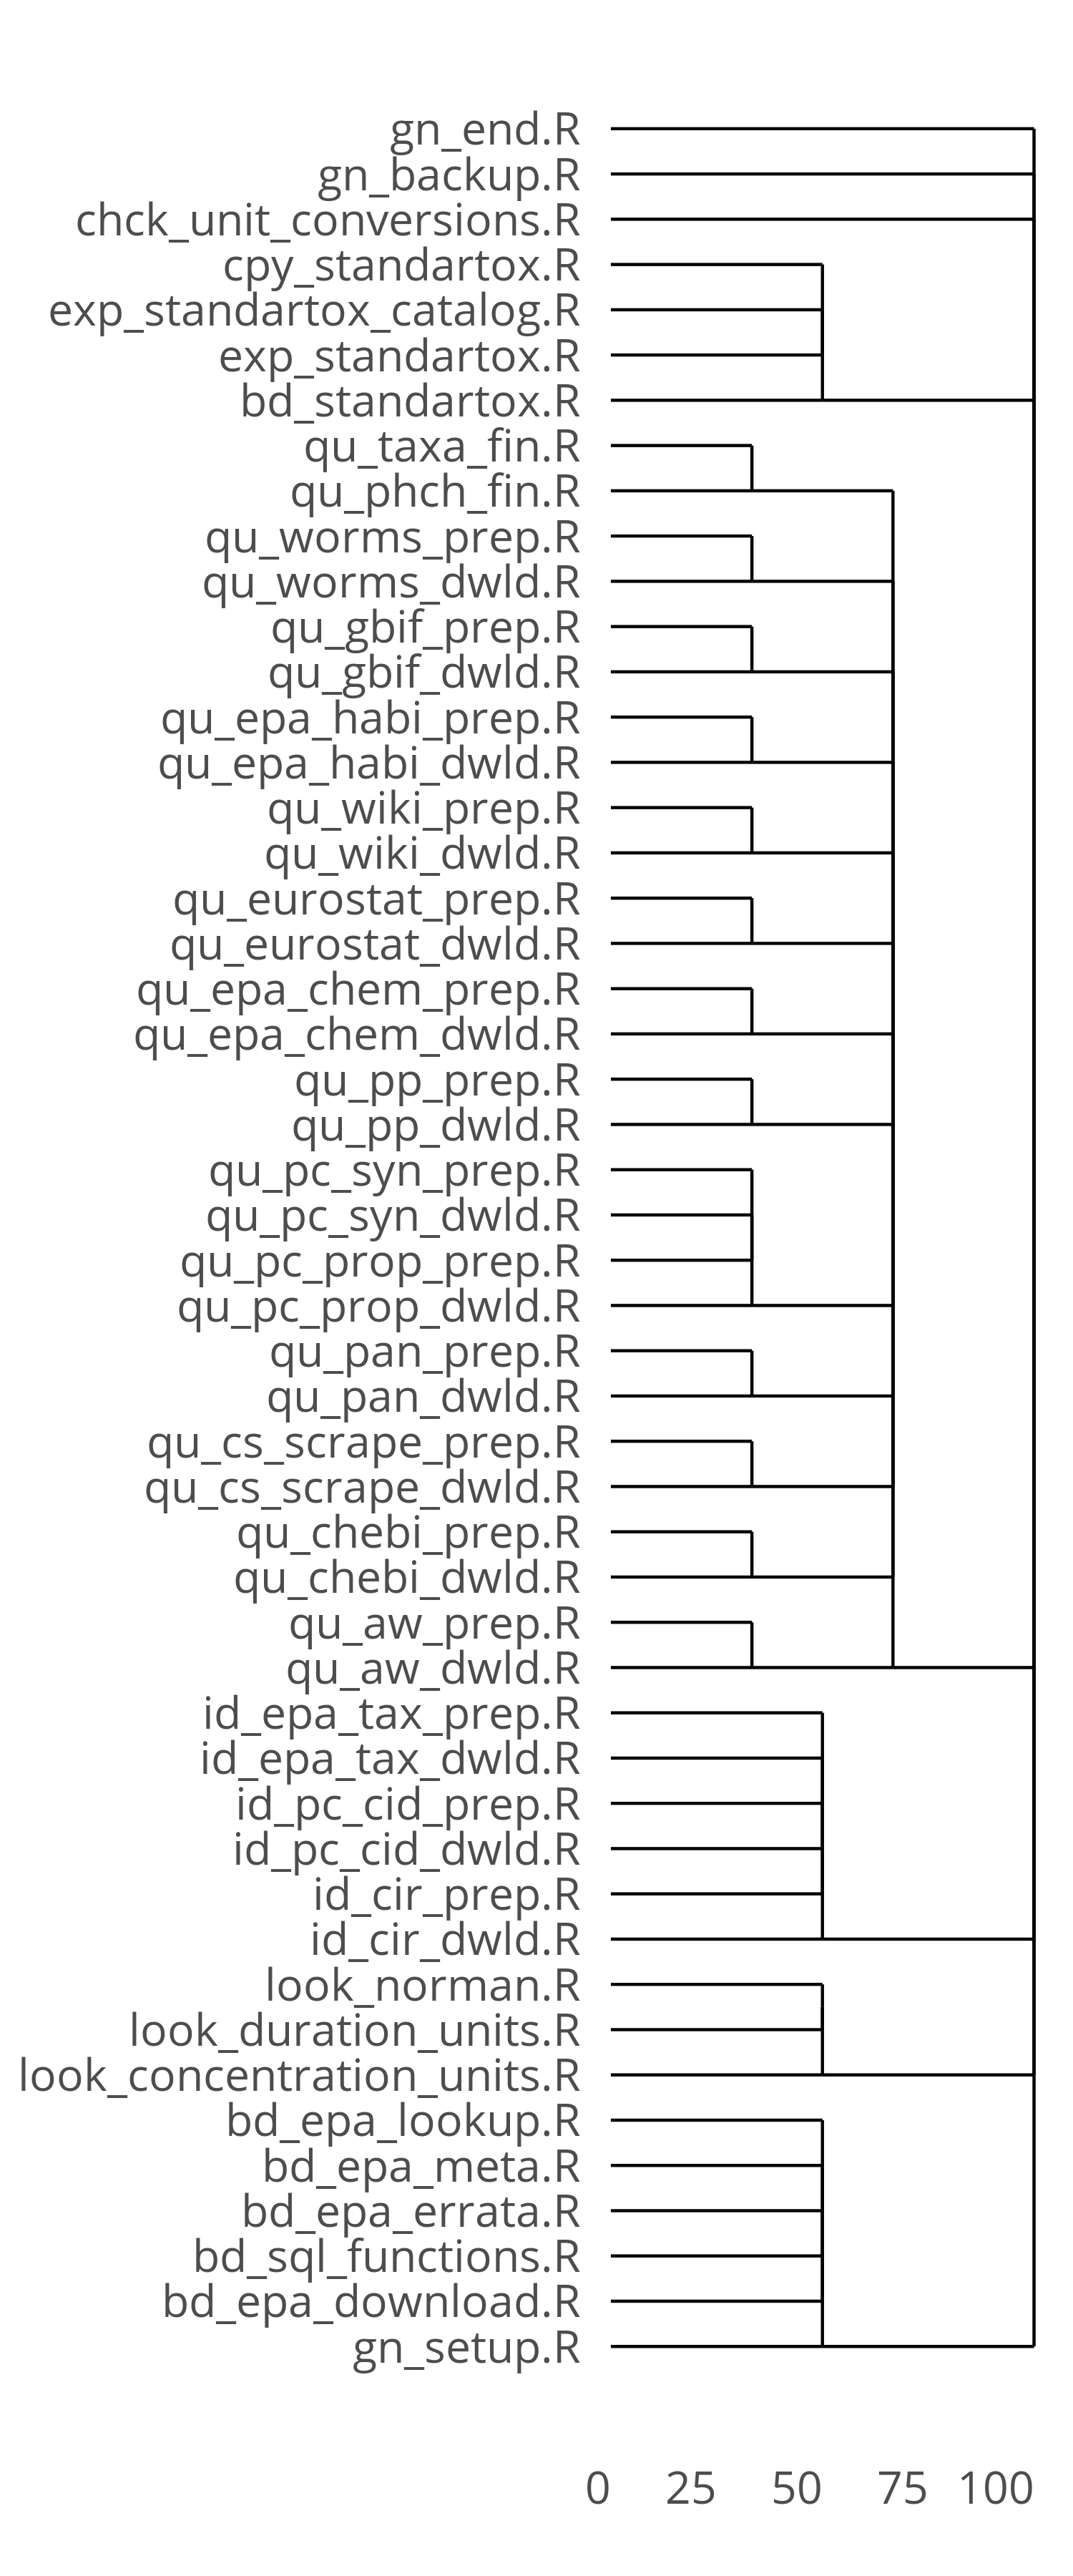
\includegraphics[width=0.5\linewidth]{article/figures/scripts_dendrogram.png}
    \caption{Processing pipeline}
    \label{fig:pipeline-tree}
\end{figure}





\end{document}







